\documentclass[pdflatex,compress,mathserif]{beamer}

%\usetheme[dark,framenumber,totalframenumber]{ElektroITK}
\usetheme[darktitle,framenumber,totalframenumber]{ElektroITK}

\usepackage[utf8]{inputenc}
\usepackage[T1]{fontenc}
\usepackage{lmodern}
\usepackage[bahasai]{babel}
\usepackage{amsmath}
\usepackage{amsfonts}
\usepackage{amssymb}
\usepackage{graphicx}
\usepackage{multicol}
\usepackage{lipsum}
\usefonttheme[onlymath]{serif}

\newcommand*{\Scale}[2][4]{\scalebox{#1}{$#2$}}%

\setbeamertemplate{caption}[numbered]

\title{KECERDASAN BUATAN}
\subtitle{ALGORITMA GENETIKA}

\author{Mifta Nur Farid}
\date{25 Januari 2024}

\begin{document}

\maketitle

\begin{frame}{Kecerdasan Buatan}
	\begin{figure}
		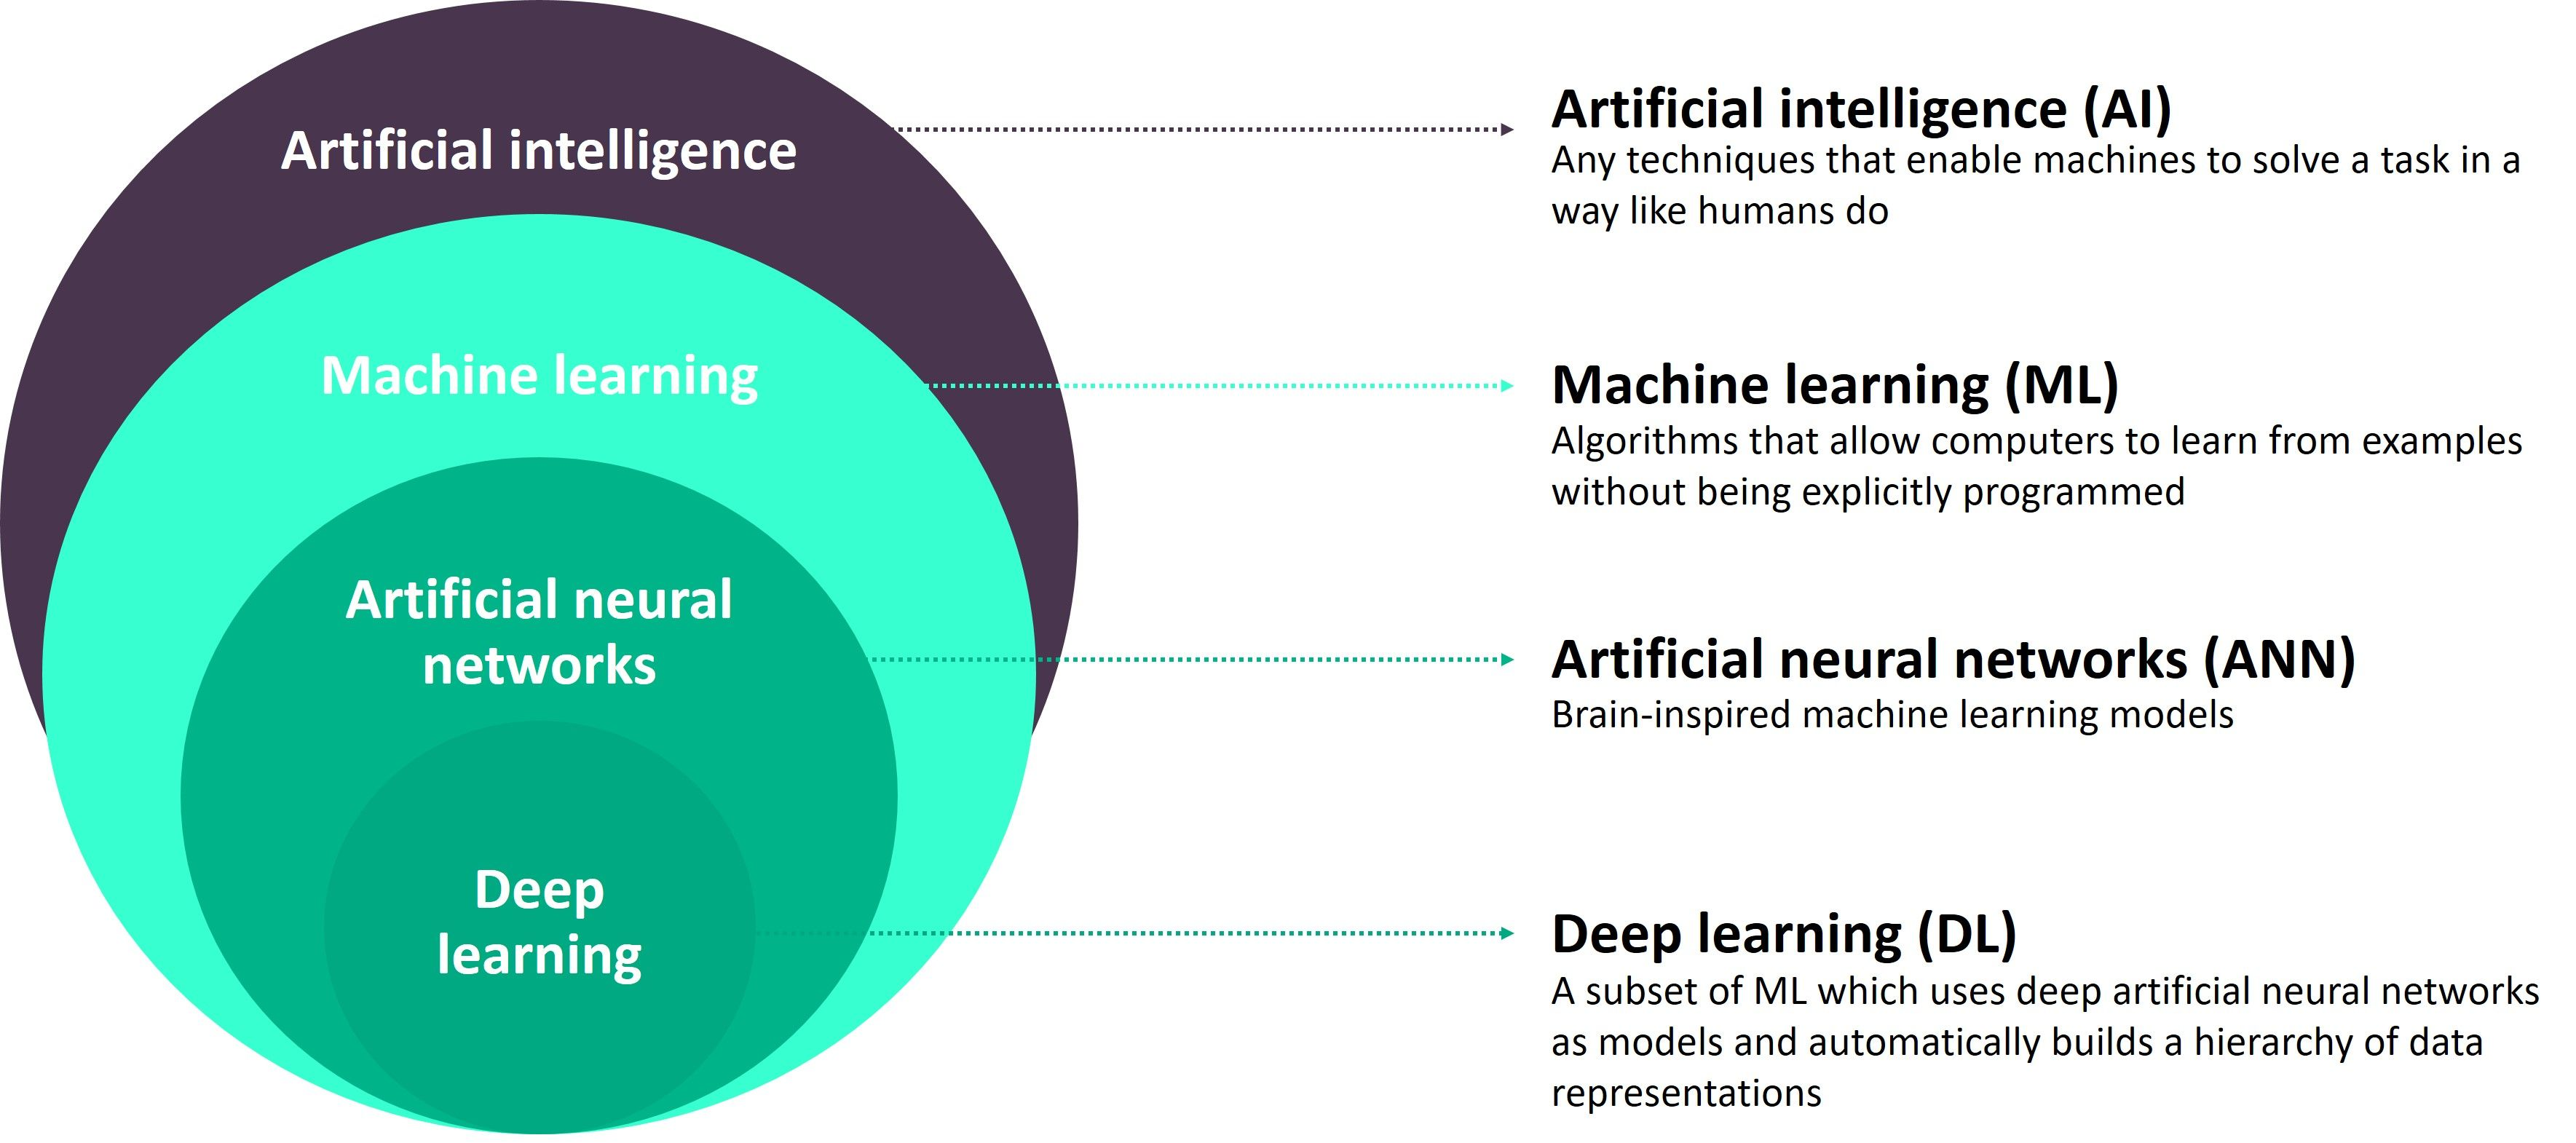
\includegraphics[width=\linewidth]{img/01}
	\end{figure}
\end{frame}

\begin{frame}{Apa yang akan kita pelajari?}
	\begin{itemize}
		\item Genetic Algorithm
		\item Particle Swarm Optimization
		\item Fuzzy Logic
		\item Neural Network
		\begin{itemize}
			\item Regression problem
			\item Classification problem
		\end{itemize}
	\end{itemize}
\end{frame}

\begin{frame}{Metode perkuliahan}
	\begin{itemize}
		\item Materi (Konsep + \emph{Coding}) akan diberikan sebelum UTS
		\item Menggunakan pemrograman python
		\item Setelah UTS diberikan project per kelompok
	\end{itemize}
\end{frame}

\begin{frame}{Algoritma Genetika / \\Genetic Algorithm (GA)}
	\begin{itemize}
		\item \textbf{Secara Umum:} Algoritma untuk memecahkan masalah tertentu yang merupakan bagian dari \emph{Artificial Intelligence}.
		\item Masalah-masalah yang bisa dipecahkan adalah dengan mencari nilai yang paling optimal dengan \textbf{CEPAT}.
		\item Sesuai namanya, GA terinspirasi dari konsep genetika pada \textbf{teori Evolusi}
	\end{itemize}
\end{frame}

\begin{frame}{Terminologi penting}
	\begin{itemize}
		\item Populasi
		\item Kromosom
		\item Gen
		\item Mutasi
		\item Fitness
	\end{itemize}
\end{frame}

\begin{frame}{Crossover (mating)}
	\begin{itemize}
		\item \textbf{Tujuan:} Menghasilkan generasi baru (anak) uang mewarisi sebagian gen dari orang-tuanya
		\item Ada 3 metode:
		\begin{enumerate}
			\item \emph{Single point}: 1 atau lebih gen di paling kiri atau kanan
			\item \emph{Double point}: 1 atau lebih gen di tengah
			\item \emph{Uniform}: 1 atau lebih gen di posisi mana saja
		\end{enumerate}
	\end{itemize}
\end{frame}

\section{My section}
\subsection{My subsection}

% ----------------------------------------------------------------------------
% *** Test frame <<<
% ----------------------------------------------------------------------------
\begin{frame}
\frametitle{A first test frame}
\lipsum[1]
\end{frame}
% ----------------------------------------------------------------------------
% *** END of Test frame >>>
% ----------------------------------------------------------------------------

% ----------------------------------------------------------------------------
% *** Test frame with overflow <<<
% ----------------------------------------------------------------------------
\begin{frame}
\frametitle{Test frame with overflow}
\lipsum%
\end{frame}
% ----------------------------------------------------------------------------
% *** END of Test frame >>>
% ----------------------------------------------------------------------------


% ----------------------------------------------------------------------------
% *** Test frame with overflow <<<
% ----------------------------------------------------------------------------
%\begin{frame}
%\frametitle{The is a test frame with a pretty long frame title}
%\lipsum
%\end{frame}
% ----------------------------------------------------------------------------
% *** END of Test frame >>>
% ----------------------------------------------------------------------------

\subsection{My subsection 2}
% ----------------------------------------------------------------------------
% *** Test frame with Itemize <<<
% ----------------------------------------------------------------------------
\begin{frame}
\frametitle{Test frame with itemize}

\begin{itemize}
    \item<1-> firstly
    \item<2-> secondly
        \begin{itemize}
            \item sub-item
            \item another sub-item
        \end{itemize}
      \item<3-> thirdly
\end{itemize}

\end{frame}
% ----------------------------------------------------------------------------
% *** END of Test frame with Itemize >>>
% ----------------------------------------------------------------------------


% ----------------------------------------------------------------------------
% *** Test frame with Math <<<
% ----------------------------------------------------------------------------
\begin{frame}
\frametitle{A math frame}

\begin{theorem}[Pythagoras]
The square of the hypotenuse of a \alert{right} triangle is equal to the sum of the squares on the other two sides:
\[
a^2 + b^2 = c^2.
\]
\end{theorem}
\begin{proof}
Straightforward.
\end{proof}

\end{frame}
% ----------------------------------------------------------------------------
% *** END of Test frame with Math >>>
% ----------------------------------------------------------------------------


% ----------------------------------------------------------------------------
% *** Test frame with Environments <<<
% ----------------------------------------------------------------------------
\begin{frame}
\frametitle{Environments}

\begin{definition}
A \textbf{prime number} (or a prime) is a natural number which has exactly two distinct natural number divisors: 1 and itself.
\end{definition}

\begin{exampleblock}{Example}
The first five prime numbers are $2$, $3$, $5$, $7$, and $11$.
\end{exampleblock}

\begin{alertblock}{Alert block}
Note that $1$ is not a prime number.
\end{alertblock}

\end{frame}
% ----------------------------------------------------------------------------
% *** END of Test frame with Environments >>>
% ----------------------------------------------------------------------------


\end{document}
